\section{KKT and Lagrange Duality}

\subsection{Example}

Optimization problem:
$\min _{x \in \mathbb{R}^2} f(x)$ s.t. $h(x)=0$

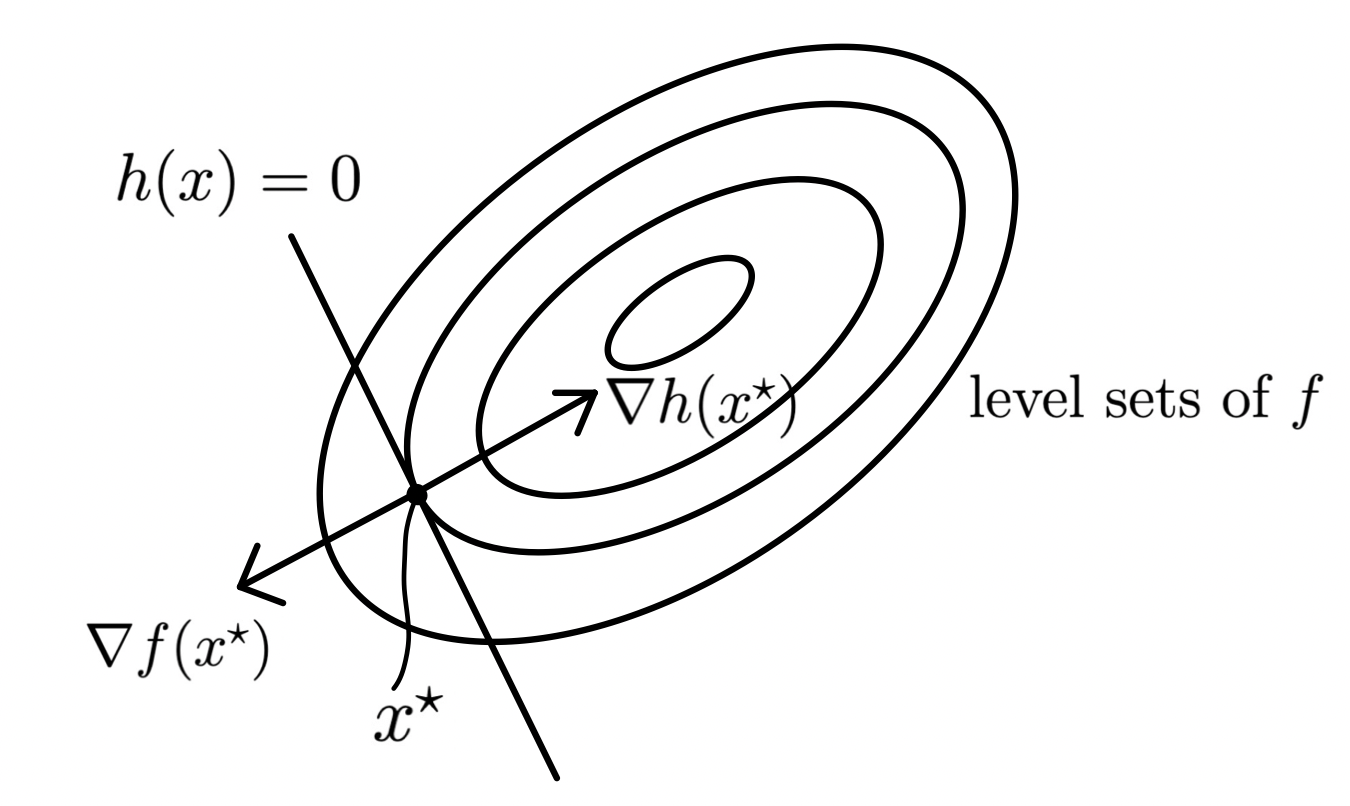
\includegraphics[width=\columnwidth]{images/op_eq_constraints.png}

We note the following:
$\nabla f(x^\star)$ and $\nabla h(x^\star)$ are colinear


$\Leftrightarrow$
$\exists\ \nu^\star \in \mathbb{R}: \nabla f(x^\star)+\nu^\star\nabla h(x^\star) = 0$

$\Leftrightarrow$
$f(x)+\nu^\star h(x)$ is stationary at $x^\star$,
where $\nu^\star$ can be interpreted as cost of violationg constraint

\subsection{Generalization}

Generalization to $n \ge 2$ and presence of inequality constraints

\begin{equation}
	f^\star = \underset{x \in \mathcal{\mathbb{R}}^n}{inf}f(x) \text{ s.t. } h(x)=0,\ g(x) \le 0
	\label{eq:dual}
\end{equation}

with corresponding Lagrange function
\begin{equation}
	\mathcal{L}(x,\lambda,\nu) = f(x) + \lambda\T g(x)+\nu\T h(x)
\end{equation}

where $\lambda_i \ge 0, \nu_i \in \mathbb{R}$ are the dual variables or multipliers
that can be interpreted as cost for violationg constraints.

\begin{proposition}[Weak Duality]
	The  dual function

	$d(\lambda,\nu) = \underset{x \in \mathcal{\mathbb{R}}^n}{inf}\mathcal{L}(x,\lambda,\nu)$ satisfies

	$d(\lambda,\nu)\le f^\star,\ \forall \lambda\ge 0,\ \nu \in \mathbb{R}^{n_h}$

\end{proposition}

\begin{proof}
	%TODO: Proof
\end{proof}

\begin{definition}[Constraint  qualification]
	$\mathcal{C}$ convex, Slaters Condition holds if
	$\exists\ \hat{x} \in \mathbb{R}^{n}$ s.t. $h(\hat{x})=0$ and $g(\hat{x})<0$
\end{definition}

\begin{proposition}[Strong Duality]
	If Slater's condition holds and (\ref{eq:dual}) is convex then
	$\exists \lambda \ge 0, \nu \in \mathbb{R}^{n_h}$ s.t. $d(\lambda,\nu)=f^\star$
\end{proposition}

\begin{proof}
	%TODO: Proof
	GRAPHIC
\end{proof}

\subsection{KKT}

$$\begin{aligned}
		\text{KKT-1 }
		 & \nabla_x\mathcal{L}(x^\star,\lambda^\star,\nu^\star)=0
		\quad \text{(Stationary\ Lagrangian)}
		\\
		\text{KKT-2 }
		 & g(x^\star)\le0, h(x^\star)=0
		\quad \text{(primal\ feasibility)}
		\\
		\text{KKT-3 }
		 & \lambda^\star\le0, \nu^\star \in \mathbb{R}^{n_h}
		\quad \text{(dual\ feasibility)}
		\\
		\text{KKT-4 }
		 & {\lambda^\star}\T g(x^\star)=0, {\nu^\star}\T h(x^\star)=0
		\quad \text{(complmntry slackness)}
		\\
	\end{aligned}$$
In addition we have:
$\sup_{\lambda\ge0,\nu\in\mathbb{R}^{n_h}}q(\lambda,\nu)=\inf_{x\in\mathcal{C}}f(x)$
\end{theorem}

QUESTION Proof?

\textbf{Remark} Without Slater,
KKT 1 to 4 still implies $x^\star$ minimizes (\ref{eq:dual})
and (\lambda,\nu) maximizes the dual,
but the converse is no longer true,
there can be primal/dual minimizer maximizer that do not satisfy KKT1-4

FORCE BALLANCE %todo

\subsection{What if $f, g$ not differentiable?}

\textbf{Example} $\underset{x \in \mathcal{\mathbb{R}}^n}{inf}|Ax -b|^2 + |x|_1$

where $\mathcal(l_1)$-norm not  differentiable at 0

\subsection{Subdifferential}

for  convex  f... %todo

\begin{definition}
	$f: \mathbb{R}^{n} \rightarrow \bar{\mathbb{R}}$ convex,
	the subdifferential of $f$ at $\bar{x}$ is:
	$\partial f(\bar{x}):= \{\lambda \in \mathbb{R}^{n} \mid f... \}$ %todo
\end{definition}

\begin{proposition}[]
	$f: \mathbb{R}^{n} \rightarrow \mathbb{R}$ convex.
	$x^\star \in argmin...$
\end{proposition}

\begin{proposition}[Relation to conjugate functions]
	$f$ convex, $epi(f)$ closed:
	$y \in \partial f(x) \leftrightarrow x \in \delta f^\star(y)$
\end{proposition}


